\chapter{Introduzione}

\section{Malware e tipologie}
Nell'ambito della sicurezza informatica, un malware è definito come un software che attua comportamenti malevoli contrari alla volontà dell'utente finale con lo scopo di modificare il normale funzionamento di un sistema, a illegittimo vantaggio del suo autore e ai danni dell'utente \cite{malwarebytes_malware_definition}.

Possono essere di varie tipologie, o unioni di alcune di esse:
\begin{itemize}
    \item \textbf{Adware}: progettati per presentare messaggi pubblicitari e guadagnare da essi
    \item \textbf{Spyware}: hanno lo scopo di osservare le azioni dell'utente senza il suo permesso per poi riportare il tutto all'autore
    \item \textbf{Virus}: vanno ad alterare altri programmi agganciandoci del proprio codice
    \item \textbf{Worm}: alterano altri computer in una stessa rete, provocando danni
    \item \textbf{Trojan}: ingannano l'utente presentandosi come un software utile, che quindi l'utente va ad installare volontariamente, non sapendo cosa si cela realmente al contrario di ciò che gli è stato promesso
    \item \textbf{Ransomware}: guadagnano sul malcapitato criptando tutti i propri file importanti, chiedendo poi un riscatto in criptovalute per lo sblocco - qui si fa leva sull'importanza e l'assenza di backup di dati importanti e sul proprio valore sia economico che morale (a seconda che si tratti di un'azienda o di un utente domestico)
    \item \textbf{Rootkit}: sfruttano vulnerabilità nel sistema target per ottenere privilegi da amministratore
\end{itemize}
Com'è normale pensare, non esistono solo questi tipi, ma sono solo alcuni dei più famosi.

Infine, per maggiore comprensione delle seguenti illustrazioni, è bene spiegare altri pochi termini:
\begin{itemize}
    \item Una \textbf{vulnerabilità} è rappresentata da una criticità in un componente di un sistema informatico, come l'assenza di misure di sicurezza o la propria compromissione
    \item Un \textbf{exploit} invece è un software o un insieme di comandi che vanno a sfruttare la vulnerabilità a proprio vantaggio, al fine di provocare un comportamento altrimenti inaspettato
    \item Un tipo particolare di exploit chiamato \textbf{zero-day} va a sfruttare falle non note prima dell'attacco, provocando così potenzialmente molti più danni, non essendo ancora disponibile una patch del software vulnerabile
    \item Per \textbf{IoC} si intende un Indicator of Compromise, indicatore usato per identificare indirizzi IP o nomi di dominio di C\&C, hash di file, firme di antivirus, o altro, che faccia ricondurre con alta probabilità a una specifica intrusione
\end{itemize}

\subsection{MITRE ATT\&CK}
\label{chap:mitre_attack}

\begin{figure}[htbp]
    \centering
    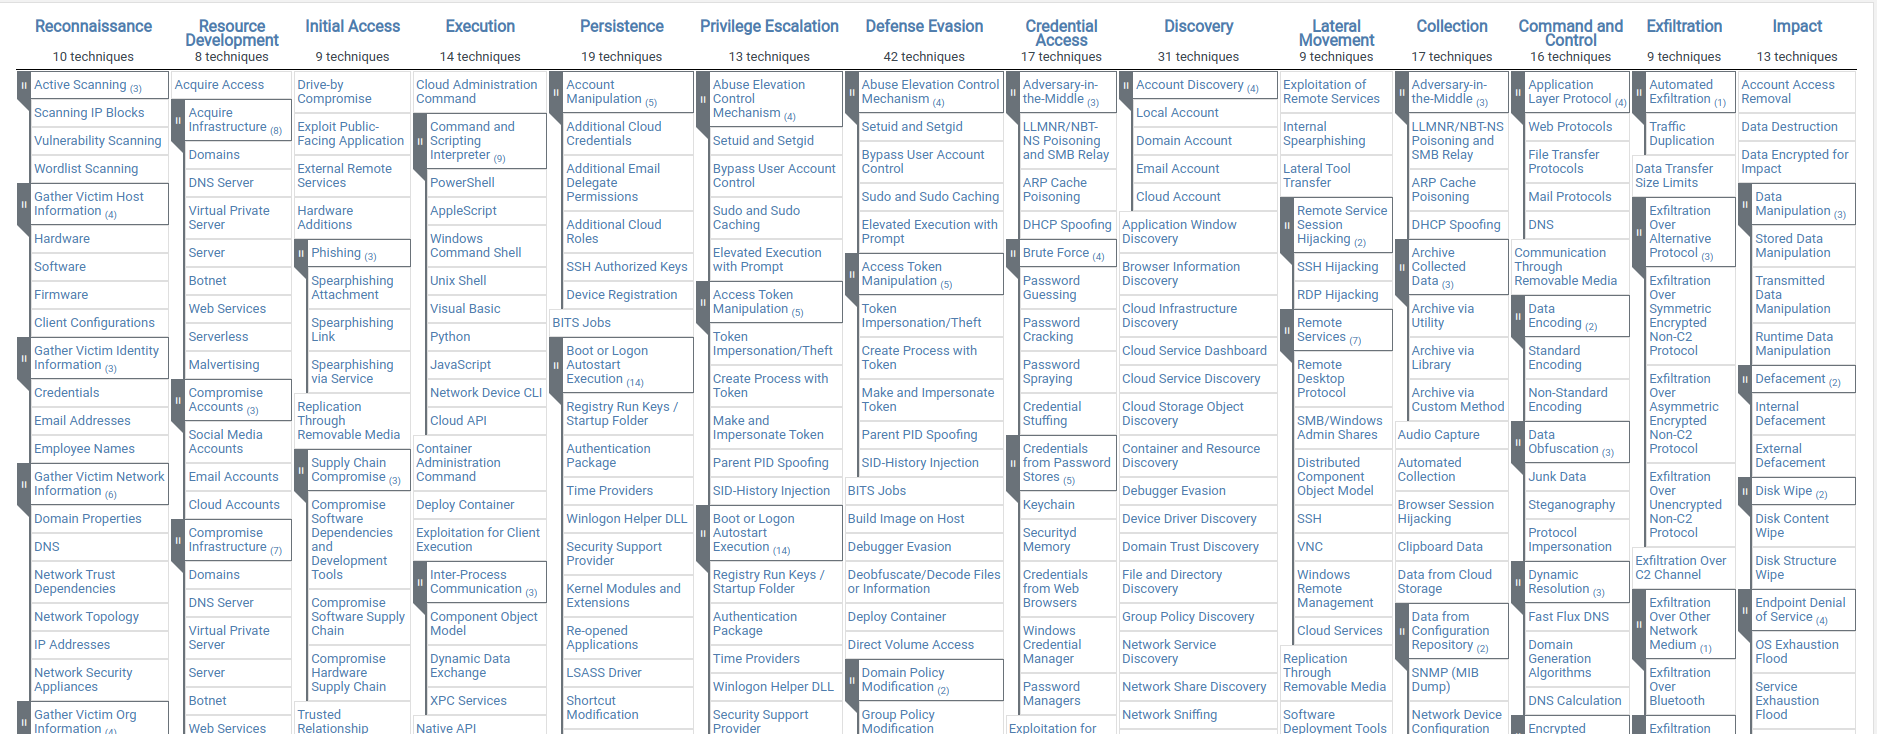
\includegraphics[width=\textwidth]{assets/mitre_attack_matrix.png}
    \caption{MITRE ATT\&CK Matrix for Enterprise}
    \label{fig:mitre_attack_matrix}
\end{figure}

Per identificare più precisamente le tipologie di malware che stiamo trattando, si va ad usare il \emph{MITRE ATT\&CK® Framework} (Adversarial Tactics, Techniques, and Common Knowledge)
\footnote{Pagina ufficiale MITRE ATT\&CK: \url{https://attack.mitre.org/}}.

Si tratta di una base di conoscenza sviluppata da MITRE Corporation, che include tattiche e adversary techniques, basata osservando gli avvenimenti nel mondo reale. Nato nel 2013 con lo scopo di descrivere le più comuni tattiche, tecniche e procedure \emph{(TTP)} usate nei sistemi Windows enterprise, ad uso interno MITRE, è poi diventato lo standard de-facto per la descrizione di tali aspetti di un attacco
\cite{mitre_attack_framework_introduction}, per far fronte all'assenza di una tassonomia comune per la descrizione dei TTP.

Si focalizza sulle interazioni che il malware ha col sistema target, e raggruppa questi comportamenti in tattiche per fornire più contesto sulla tecnica utilizzata.
\begin{itemize}
    \item Le tattiche sono il \emph{perché} di una tecnica, indicando l'obiettivo che si intende perseguire, e servono da contenitore per le varie tecniche; nello standard iniziano per \texttt{TA} (es: \texttt{TA0043} - Reconnaissance - Ricognizione, l'avversario va ad ottenere informazioni sul sistema per capire come muoversi)
    \item Le tecniche invece sono il \emph{come} di una specifica azione, e potrebbero far dedurre anche il \emph{cosa} un avversario ottiene come risultato della sua azione - particolarmente utile nella tattica TA0007 Discovery, dove si cerca di studiare la composizione del sistema target. \\
    Una tecnica è spesso composta da sotto-tecniche per essere ancora più specifici.
    Ad esempio, la tecnica \texttt{T1595.002} Vulnerability Scanning (dove si va capendo i software disponibili sul sistema target e la loro versione, con il possibile scopo di verificare se si allinea a una specifica versione vulnerabile di cui l'avversario già dispone di un exploit) è sotto-tecnica di \texttt{T1595} Active Scanning, e fa parte della tattica \texttt{TA0043} Reconnaissance vista al punto precedente.
\end{itemize}

Nella matrice in figura \ref{fig:mitre_attack_matrix}, le tattiche sono le colonne e le tecniche sono le celle, possibilmente composte da sotto-tecniche.

Viene usato anche per l'integrazione con la Cyber Threat Intelligence, che vedremo nella sezione \ref{chap:cyber_threat_intelligence}, punto focale anche degli strumenti realizzati nel progetto.

\section{Cyber Kill Chain}
Partendo dalle tattiche appena viste, possiamo costruire ciò che è noto col nome di \emph{Cyber Kill Chain}.
Si tratta di un modello simile al MITRE ATT\&CK framework (sez. \ref{chap:mitre_attack}), ma segue un diverso approccio. Qui infatti si vanno a ripercorrere le 7 tipiche fasi cronologiche di un attacco ad un sistema informatico, fornendo una panoramica più ad alto livello.

\begin{figure}[h]
    \centering
    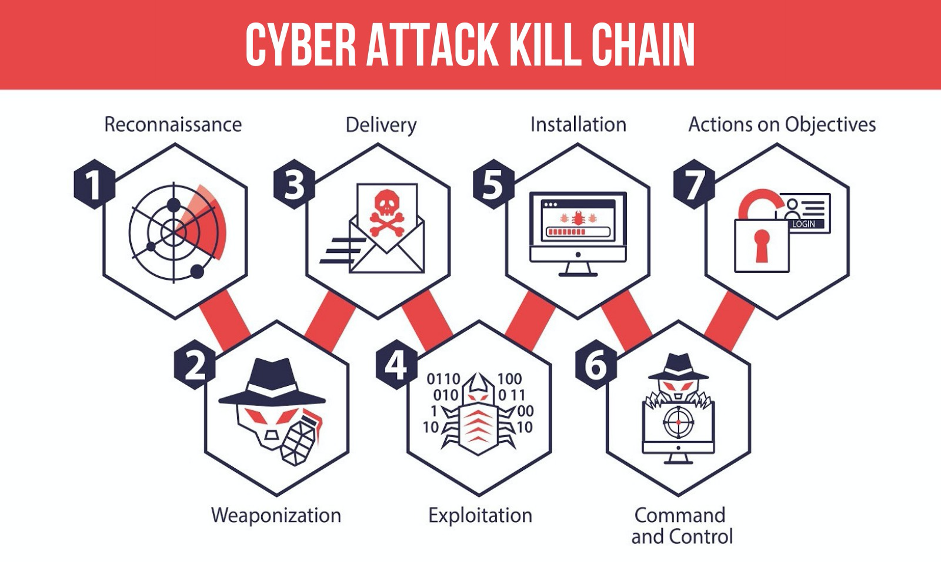
\includegraphics[width=0.6\textwidth]{assets/cyber_kill_chain.png}
    \caption{(diritti di uso dell'immagine concessi dall'autore "Fondazione F3RM1")}
    \label{fig:cyber_kill_chain}
\end{figure}

Si compone delle seguenti fasi \cite{cyber_kill_chain_360}, portando un esempio noto, alla base anche della challenge \emph{Pilgrimage} della piattaforma \emph{HackTheBox}:
\begin{enumerate}
    \item \textbf{Ricognizione}: identificazione dei punti di accesso a un sistema e sue vulnerabilità, derivabili tramite analisi attiva (uso di strumenti come \emph{nmap} in maniera più o meno aggressiva) o passiva, leggendo informazioni già da fonti note (come \emph{Shodan.io} partendo da un indirizzo IP): nell'esempio notiamo che è esposta la cartella .git della Git repository, da cui estraiamo il sorgente della webapp, trovando l'uso di ImageMagick 7.1.0-49
    
    \item \textbf{Armamento}: creazione del vero e proprio malware da utilizzare nell'attacco, nell'intento di sfruttare la vulnerabilità individuata - nell'esempio creiamo la nostra immagine PNG ad-hoc

    \item \textbf{Consegna}: il payload creato deve essere consegnato alla vittima in qualche modo, come una mail di phishing o un form di una pagina del sito web - quindi eseguiamo l'upload del PNG nel form dal sito

    \item \textbf{Exploit}: nella realtà dei fatti, si sta sfruttando una vulnerabilità individuata - nel nostro caso reale, sfruttiamo la CVE-2022-44268 e leggiamo il file del database della webapp, incluse le password

    \item \textbf{Installazione}: dopo la riuscita dell'exploit, si scarica e avvia il payload malevolo, cercando di bypassare strategie esistenti di rilevazione, usando metodologie come obfuscation - nell'esempio, accediamo via SSH con la password e possiamo installare il nostro sistema

    \item \textbf{Command and Control (C\&C)}: andiamo a instaurare un canale di comunicazione tra noi e la vittima, così da controllarlo da remoto - la forma più basilare è l'avvio di una Reverse Shell criptata

    \item \textbf{Azioni sugli obiettivi}: eseguiamo le azioni più disparate, in base a ciò che vogliamo fare noi come attaccanti - nella CTF, andremo a leggere un file contenente il flag, simbolicamente un dato sensibile sul sistema della vittima
\end{enumerate}

\section{Tipi di sistemi di protezione}
Antivirus, EDR, XDR

\subsection{Come funziona la sicurezza nelle aziende}
\begin{itemize}
    \item IDS, IPS 
    \item https://www.youtube.com/watch?v=j7Cu0lxjW-o
    \item Ruolo degli Agent e altri sistemi
\end{itemize}

\section{Cyber Threat Intelligence}
\label{chap:cyber_threat_intelligence}

\section{Ruolo ricoperto dall'azienda}

\section{Il problema}
Gyala Products (Endpoint, Network Probes, Mobile Agent) need a capability to enable detection of both unauthorised and malicious behaviours.
The ability of perform high quality detection is one of the distinctive trait between different security solutions and has a direct repercussion to customer satisfaction and brand reputation.  
Malware Analysis should be considered an integrated, as part of product development, and continuous process that adds value in gyala products and makes them effective and distinctive on the market.

lo scopo è ridurre i costi di virustotal, che si usa tantissimo, e potenziare il set di strumenti a disposizione dell'analista, potenzialmente integrandoli tutti in uno con sistema di plugin